\documentclass[fleqn,twoside]{article}
\usepackage{espcrc2}

%\documentclass{elsart}

%\usepackage{elsart12}
% Use the option doublespacing or reviewcopy to obtain double line spacing
% \documentclass[doublespacing]{elsart}

% the natbib package allows both number and author-year (Harvard)
% style referencing;
%\usepackage{natbib}
%%\documentclass{article}
\usepackage{amsmath,amssymb}
\usepackage{graphicx,subfigure}


% if you want to include PostScript figures
\usepackage{graphicx}
% if you have landscape tables
\usepackage[figuresright]{rotating}



\bibliographystyle{plain}%elsart-harv}


\newtheorem{defi}{Definition}
\newtheorem{prop}{Proposition}
\newtheorem{theo}{Theorem}
\newtheorem{lem}{Lemma}

\newcommand{\ttbs}{\char'134}
\newcommand{\AmS}{{\protect\the\textfont2
  A\kern-.1667em\lower.5ex\hbox{M}\kern-.125emS}}

% add words to TeX's hyphenation exception list
\hyphenation{author another created financial paper re-commend-ed Post-Script}

% declarations for front matter
\title{2D and 3D Visibility in Discrete Geometry: an application to  discrete geodesic paths}

\author{D. Coeurjolly\address[ERIC]{Laboratoire ERIC\\ Universit{\'e} Lumi{\`e}re Lyon 2\\ 5,  av. Pierre Mend{\`e}s-France \\ 69676 BRON cedex, FRANCE}, S. Miguet\addressmark[ERIC] and L. Tougne\addressmark[ERIC]}
       
       
\begin{document}

\begin{abstract}
In this  article, we present  a discrete  definition of the  classical
visibility in computational geometry  based on digital straight lines.
We   present efficient algorithms to  compute  the set  of pixels in a
non-convex domain  that are  visible from a  source pixel.    Based on
these   definitions, we define   discrete geodesic  paths  in discrete
domain with obstacles.  This allows   us to introduce a new   geodesic
metric in discrete geometry.  \vspace{1pc}
\end{abstract}

% typeset front matter (including abstract)
\maketitle


%\begin{document}
%\begin{frontmatter}
%\title{Visibility in Discrete Geometry: an application to discrete geodesic paths}
%\author{David Coeurjolly}
%\ead{david.coeurjolly@univ-lyon2.fr}
%\author{Serge Miguet}
%\ead{serge.miguet@univ-lyon2.fr}
%\author{Laure Tougne}
%\ead{laure.tougne@univ-lyon2.fr}


%\address{ Laboratoire ERIC\\ Universit{\'e} Lumi{\`e}re Lyon 2\\ 5,
%  av. Pierre Mend{\`e}s-France \\ 69676 BRON cedex, FRANCE}
%% \title{Title\thanksref{label1}}
%% \thanks[label1]{}
%% \author{Name\corauthref{cor1}\thanksref{label2}}
%% \ead{email address}
%% \ead[url]{home page}
%% \thanks[label2]{}
%%corauth[cor1]{coucou}
%% \address{Address\thanksref{label3}}
%% \thanks[label3]{}





%\begin{abstract}
%In this article,  we present  a  discrete definition of the  classical
%visibility in computational geometry based  on digital straight lines.
%We present efficient algorithms  to compute the set  of  pixels in a non-convex
%domain  that  are visible  from  a   source  pixel.   Based on   these
%definitions, we define discrete geodesic paths in discrete domain with
%obstacles.  This allows  us  to introduce  a  new  geodesic metric  in
%discrete geometry.
%\end{abstract}

%\begin{keyword}
%discrete visibility \sep geodesic distance

%% keywords here, in the form: keyword \sep keyword

%% PACS codes here, in the form: \PACS code \sep code

%\end{keyword}


%\end{frontmatter}

\section{Introduction}

In discrete geometry, many Euclidean  geometric tools are redefined to
take   into  account  specificities  of  the  discrete  grid.  In this
article, we propose a definition of the classical Euclidean visibility
based on  discrete  objects.  The interest  is double:  on one hand we
extend  the discrete geometry  with a new tool and  on the other hand,
since this visibility allows us to  define discrete geodesic paths and
discrete  shortest  paths, we have a   practical  tool needed  by many
applications in medical imaging or image analysis to estimate geodesic
distance in non-convex domains.

In the  literature, Soille \cite{soille91,soille94,soillebook}    defines the
visibility between two   points  using the Bresenham   digital line
drawing algorithm \cite{bres65}. The  visibility definition we
propose  in this article is based on
classical   Discrete Straight Lines  (DSL  for short).  Hence the
proposed approach considers a more general set of lines and allows
efficient algorithms.
Many technics
exist for the  DSL recognition problem. Some  of these  approaches are
based on chain code  analysis \cite{wu}, on  links between the  chain
code and arithmetical properties of DSL \cite{DEB95b,DEB95}, on links
between the chain   code and  the  feasible  region in  the dual   -or
parameter- space \cite{dor91,bruck93,vittone}  and  others  on linear
programming      tools    such     that  Fourier-Motzkin's   algorithm
\cite{fourier}.  All these algorithms  present  a solution either  to
decide if a given  set of pixels is a  discrete straight  segment (DSS
for short) or  to segment a discrete curve  into DSS, or  both. In our
case, the problem is quite different, we want to decide if there exits
at least one DSS between two pixels in a non-convex domain.

We present  definitions and  algorithms to  compute  the set of pixels
which are visible from a source.  Then, we define the  notion of discrete
geodesic path  and  the  metric associated to  such   path based on  this
visibility definition. We also proposed an efficient implementation of
the geodesic distance labelling from a source pixel. In section
\ref{section3D}, we present some ideas for a 3D generalization.


\section{Visibility}

\subsection{Notions and definitions}

Let  us denote  $\mathcal{D}$   a {\it  discrete   domain}, that is  a
$n-$connected set   of  pixels.    We denote  $\bar{\mathcal{D}}$  the
complement of $\mathcal{D}$, we  call this set indifferently  the {\it
background} or the   {\it  set of  obstacles}.  In  the following,  we
consider $\mathcal{D}$ a 8-connected domain.

In this domain, we define the discrete visibility by analogy to the continuous definition.

\begin{defi}[Discrete Visibility]
Let $s$ and $t$ be two pixels in $\mathcal{D}$, we define the discrete
visibility       as        a     binary          relationship      $v \subseteq
\mathcal{D}\times \mathcal{D}$ such that we  have $v(s,t)$  if and
only if there exists a  8-connected discrete straight segment from $s$
to $t$ whose pixels belong to $\mathcal{D}$
\end{defi}

Before introducing the   visibility problem in  non-convex domain,  we
recall   classical   parameter    space   characterizations   of   DSL
\cite{bruck93,ilroy,vittone}.  If we consider  an Euclidean  straight
line $y=\alpha x+\beta$, the digitization of this  line using the Grid
Intersect    Quantization (see   \cite{jonas97}   for  a  survey   on
digitization scheme) is the set of discrete points such that:
\begin{equation}
\Delta(\alpha,\beta)=\{ (x,y)\in \mathbb{Z}^2 | -\frac{1}{2}\leq\alpha x+\beta-y<\frac{1}{2}\}
\end{equation}

Note that all  classical  digitization schemes (GIQ,  Object  Boundary
Quantization or Background Boundary Quantization) can be used and such
a  choice  will not interfere  in  our  algorithms. We  choose here the GIQ
scheme because of its symmetry properties.

In the parameter space of the previous definition, we can describe the
set of Euclidean straight   lines  whose  digitization contains   a
pixel $p(x,y)$:
\begin{equation}
S_p=\{ (\alpha,\beta)\in \mathbb{R}^2 | -\frac{1}{2}+y\leq\alpha x+\beta<\frac{1}{2}+y\}
\end{equation}

A  pixel      in $\mathcal{D}$   defines  a     {\it  strip}   in  the
$(\alpha,\beta)$-space delimited by   two lines $L_1: \alpha   x+\beta
-y\geq-1/2$  and $L_2: \alpha  x+\beta -y<1/2$.  If we
want to know if a  set of pixels belongs to  a DSL, a classical way is
to compute the intersection   in the $(\alpha,\beta)$-space of  strips
associated to  each  pixel. If  the feasible  domain is not  empty, it
describes all  DSL containing the pixels  (cf figure \ref{coupures} for an
example).  In  the following, we  define the domain $\mathcal{S}(s,t)$
associated to two pixels $s$ and $t$ which is the intersection $S_s\cap S_t$.

%\begin{figure}[htbp]
%  \begin{center}
%    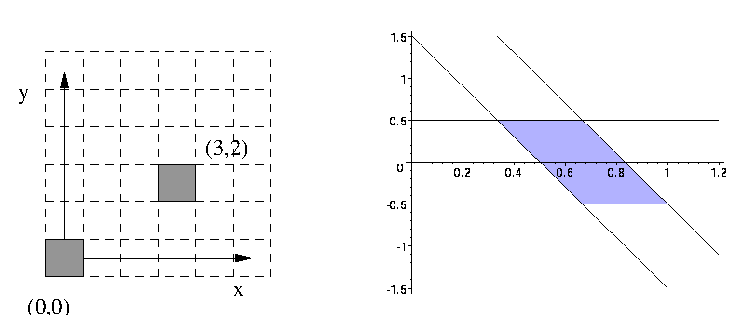
\includegraphics[width=7cm]{dual}
%    \caption{An example of $\mathcal{S}(s,t)$ domain with pixels (0,0) and (3,2), the
%      $\mathcal{S}(s,t)$ domain in the parameter space defined by inequations
% : $\{\beta <1/2,\beta\geq-1/2, \beta <-3\alpha+5/2,\beta\geq-3\alpha+3/2\}$.}
%    \label{dual}
%  \end{center}
%\end{figure}


In  order to  compute the  visibility in  non-convex domains, the main
idea is to check  in the dual  space if domains associated to obstacle
pixels do not hide the current pixel $t$ from the source $s$.





\subsection{Visibility domain}

Let $o$ denote  an obstacle pixel. If we  want to describe  the set of
Euclidean straight  lines whose digitizations  do not  contain $o$, we
also  introduce a  strip   in  the  parameter   space such   that  the
inequations  are  reversed.  Hence,  an obstacle $o$  is associated to
constraints  $\bar{L}_1(o): \alpha x+\beta -y<-1/2$ and $\bar{L}_2(o):
\alpha x+\beta -y\geq  1/2$. If we want to  know if this obstacle {\it
blocks} the visibility from $s$ to $t$, we just have to compute in the
$(\alpha,\beta)$-space $L_1(s)\cap L_2(s)\cap  L_1(t) \cap L_2(t) \cap
\bar{L}_1(o) \cap \bar{L}_2(o)$.  If  this intersection is  empty then
$t$ is not visible from $s$.


More generally, if we consider a non-convex domain $\mathcal{D}$ and a
set  of  obstacle  pixels  $\mathcal{O}=\{o_i\}_{i=1..n}$   that  is a
restriction of $\bar{\mathcal{D}}$  such that all point abscissas  are
between the abscissa of $s$ and the abscissa  of $t$ (all other points
can be omitted for the visibility problem). We have the lemma:

\begin{lem}
Let $s$ be the source and $t$ a pixel in $\mathcal{D}$, $t$ is visible
from $s$ in $\mathcal{D}$ if and only if:
\begin{equation}
  \mathcal{S}(s,t)\cap \left (  \bigcap_{i=1..n}\bar{L}_1(o_i)\cap \bar{L}_2(o_i)\right ) \neq \emptyset
\end{equation}
\end{lem}

The  proof of this lemma can  be  deduced by the visibility definition
and by construction of $\mathcal{S}$.

Obviously, we do not have to consider all obstacle pixels. We first define:
\begin{defi}
  A pixel $o$ in $\mathcal{O}$   is called ``blocking pixel'' for  the
  visibility problem $v(s,t)$ if:
  \begin{equation}
    \mathcal{S}(s,t) \cap \bar{L}_1(o)\cap \bar{L}_2(o)  \neq  \mathcal{S}(s,t)
  \end{equation}
and the abscissa of $o$ is between the abscissa of $s$ and $t$.
\label{def_b}
\end{defi}

These  blocking pixels are  those  which interfere  in  the visibility
problem. Non-blocking pixels in $\mathcal{O}$  can be removed from the
$v(s,t)$ test.   We can characterize  the shape of   the domain when a
blocking pixel modifies it:
\begin{lem}
  If $o$ is a blocking pixel for the $v(s,t)$ problem, either the  domain
  $\mathcal{S}(s,t)\cap\bar{L}_1(o)\cap \bar{L}_2(o)$  is empty or it
 has only one connected component.
\end{lem}

\noindent{\it Proof}: we consider the domain $\mathcal{S}(s,t)$ and a blocking pixel $o$ such that 
$o$, $s$ and $t$ are not aligned (in  that case, the domain is empty).
We  show that  either $\bar{L}_1(o)$   or  $\bar{L}_2(o)$ crosses  the
domain.  We  have different cases  (cf figure \ref{preuve_2_1}-a) that
induce two  components but the left  and the middle cases are excluded
because they  imply  that the  abscissa of $o$   denoted $x_o$ is  not
between  $x_s$  and $x_t$  and thus,   $o$  is  not  a  blocking pixel
according to definition \ref{def_b}.  As  the matter of fact, if $x_o$
is  between  $x_s$  and  $x_t$, then the   slope of  $\bar{L}_1(o)$ is
between the   slope  of $L_1(s)$  and   the  slope of  $L_1(t)$.    By
construction of  the strips, the vertical  distance between  $L_1$ and
$L_2$  is  equal   to 1.  Hence,   in   figure \ref{preuve_2_1}-b, the
intersection  in  $a'$ of $\bar{L}_1$   with  the vertical  line going
through $b$ implies that $b'$ must be outside  the interval $[a,b]$ on
the vertical line. Since the slope of  $\bar{L}_2$ is greater than the
slope of the edge $cb$, $\bar{L}_2$ cannot cross the domain. Same idea
can be applied when $\bar{L}_2$ crosses  the domain.  Hence, all cases
of    the  figure    \ref{preuve_2_1}-a   are   impossible  and  thus,
$\mathcal{S}(s,t))\cap\bar{L}_1(o)\cap   \bar{L}_2(o)$ has only    one
connected component. \hfill $\Box$

\begin{figure}[htbp]
  \begin{center}
    \subfigure[]{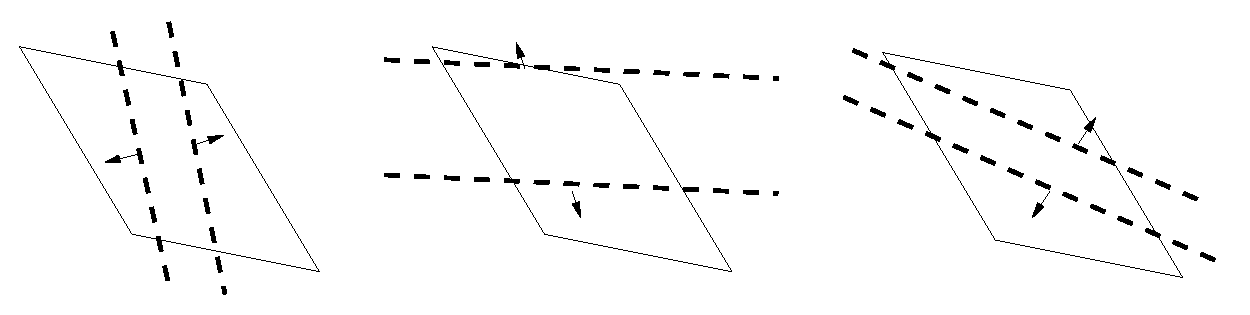
\includegraphics[width=5.25cm]{preuve_2}}
    \subfigure[]{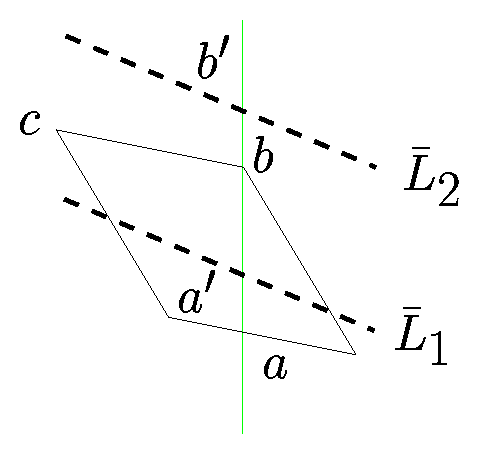
\includegraphics[width=2.1cm]{preuve_2bis.ps}}
     \caption{ (a) Different cases that induce two connected components, the left case and the middle case
      are impossible by definition  of blocking points. The third case
      must  be  taken into account  (b)  illustration of the proof of
      lemma 2.}
    \label{preuve_2_1}
  \end{center}
\end{figure}


According to  this lemma,   if   a straight  line $\bar{L}_1$   (resp.
$\bar{L}_2$)  of an obstacle crosses the  domain, the other constraint
$\bar{L}_2$ (resp.  $\bar{L}_1$)  can be  removed  for the  visibility
problem.  Geometrically, an obstacle such that $\bar{L}_1$ crosses the
domain is above  the Euclidean segment   $[s,t]$ and an obstacle  such
that $\bar{L}_2$ crosses the $\mathcal{S}(s,t)$  domain is beneath the
segment $[s,t]$ (cf figure  \ref{coupures} for an example). %We  denote
%$\mathcal{U}(s,t)$ the  set  of  blocking   pixels above  $[s,t]$  and
%$\mathcal{L}(s,t)$ the  set  of  blocking pixels  beneath  the segment
%$[s,t]$.

\begin{figure}[htbp]
  \begin{center}
    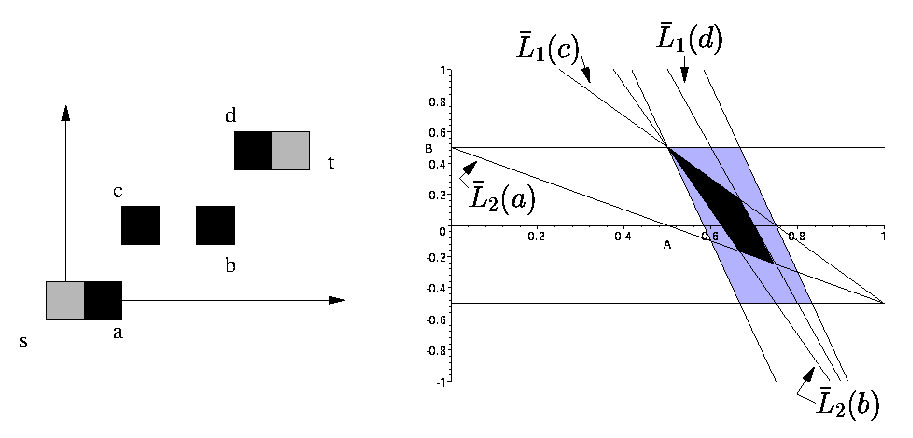
\includegraphics[width=7.5cm]{coupuresbis.ps}
    \caption{Visiblity domain associated to a set of blocking pixels. The black feasible region in
      the parameter space is the visibility domain associated to grey pixels constrained with the
      black blocking pixels.}
    \label{coupures}
  \end{center}
\end{figure}


In \cite{soille91,soille94,soillebook}, Soille computes the visibility test
considering the digitization, using the Bresenham's algorithm
\cite{bres65}, of the Euclidean segment $[st]$ and verifying that all
pixels of this segment belong to the domain. In our proposal, we
consider all possible digital straight segment and thus we increase
the visibility domain. Beyond these different definitions, we present
efficient algorithms for both visibility labelling and geodesic
distance labelling.


\subsection{Visibility algorithm}

In  this section, we  present algorithms that  compute the equivalence
class  associated to  the visibility binary  relationship  of a source
$s$.

We propose two   algorithms, the first  one   computes the equivalence
class with the  visibility definition given above,  and the second one
introduces a new visibility definition  that  is a restriction of  the
previous  one but the associated  algorithm  complexity justifies this
new version of the visibility.

The first algorithm we propose is a really straightforward computation
of the  visibility. Indeed,  we can  use classical linear  programming
tools  to solve   the   linear inequation  system    given by obstacle
constraints.    Such  tools are    for   example  the  Fourier-Motzkin
\cite{fourier} system simplification algorithm, the Simplex algorithm
or the Megiddo's algorithm \cite{megiddo}.   Note that the complexity
of the Megiddo's algorithm is linear in  the number of inequations but
the problem comes with the dimension of  the system.  In our case, the
constraint system is in dimension 2 and thus the implementation of the
Megiddo's algorithm is tractable  with  a complexity bounded  by  $4n$
where $n$ is the number of inequations.

We consider a source $s$, a  domain $\mathcal{D}$. We label all pixels
in $\mathcal{D}$  using a breadth-first tracking   of the domain using
for  example the 8-adjacency.  During the  propagation process, if  we
meet an obstacle we store its coordinates in a list $O$. At each pixel
visited in the breadth-first tracking, we  extract from $O$ the set of
blocking pixels and    we  solve the  visibility problem    using  the
Megiddo's algorithm.

\ \\
{\small \hrule 
\ \\
\centerline{\textsf{Straightforward visibility algorithm}}
{\sf
Input:~a domain $\mathcal{D}$ and a source $s$\\
Output:~the set of pixels which satisfy $v(s,t)$\\
\ \\
Let Q be a FIFO queue\\
Let O be the obstacle list\\
Append\_last(s,Q)\\
{\bf While} Q is not empty\\
\hspace*{0.5cm} t:=remove\_first(Q)\\
\hspace*{0.5cm} {\bf For each} 8-neighbor $n$ of $t$ not labelled {\tt closed} or {\tt visible}\\
\hspace*{1cm} {\bf If} $n$ is an obstacle {\bf then}\\
\hspace*{1.5cm} Append(n,O)\\
\hspace*{1cm}{\bf else}\\
\hspace*{1.5cm} Let B be the set of blocking points of O according to the pixel $n$\\
\hspace*{1.5cm} Compute the linear inequation system $S$ with $\bar{L}_1$ or $\bar{L}_2$ the
constraints of each point of B\\
\hspace*{1.5cm} {\bf If} $Megiddo(S)\neq\emptyset$ {\bf then }\\
\hspace*{2cm} Label $n$ as {\tt visible}\\
\hspace*{2cm} Append\_last(n,Q)\\
\hspace*{1.5cm}{\bf else}\\
\hspace*{2cm} Label $n$ as {\tt closed} //$n$ is not visible and the point is closed\\
\hspace*{0.5cm} {\bf endFor}\\
{\bf endWhile}\\
}
\hrule}\ \\

If  we denote $n$ the  number of pixels  in  $\mathcal{D}$ and $m$ the
number  of obstacles in $O$,  each  step in the  while  loop has got a
complexity bounded by $O(m)$. Hence, the global cost of this algorithm
is $O(nm)$.

Due  to  the difficulties to  provide an  efficient data  structure to
propagate  blocking   points  from a  point  to   its neighbors,  this
algorithm has a  quite important complexity  and is not efficient  for
the geodesic  computation.  Thus, we propose a   new definition of the
discrete    visibility  which is  a weak   version   of the definition
presented above  but  that leads  to an   efficient algorithm for  the
visibility computation and the discrete geodesic problem.

\begin{defi}[Weak Discrete Visibility]
Let $s$ and $t$ two pixels in $\mathcal{D}$, we define the weak
discrete visibility as a binary relationship $v^* \subseteq \mathcal{D}\times\mathcal{D}$ such that we have $v^*(s,t)$ if and only if 
 there exists an Euclidean straight line going through $s$ and whose digitization contains $t$ 
and no pixels in $\bar{\mathcal{D}}$ between $s$ and $t$.
\end{defi}


Instead of considering the inequation associated to $s$, we constraint
the set  of Euclidean lines to go   through $s$.  This  new definition
restricts the previous one and make the visibility  not be a symmetric
binary relationship. However, this definition allows an efficient data
structure for the visibility test.  We  suppose that all the  obstacle
pixels are sorted counterclockwise by  polar angles  using $s$ as  the
origin. Using  this data structure and  the  above definition, we have
the following property.


\begin{prop}
Given  a set of obstacles  sorted by polar angles  of center $s$ and a
point $t$, we denote $u$ the successor of $t$ in the polar sort and $l$ its
predecessor. We have:
\begin{equation}
  v^*(s,t) \Leftrightarrow \mathcal{S}^*(s,t) \cap \bar{L}_1(u) \cap \bar{L}_2(l) \neq \emptyset
\end{equation}
\end{prop}

where  $\mathcal{S}^*$ denotes the new domain   associated to the weak
visibility which is now a segment in the parameter space.

Hence, instead of  considering all  blocking pixels,  we just  have to
test  two characteristic pixels  given by  a  polar sort. The proof of
this  property is  a   straightforward application of the   visibility
definition.   Note that the   polar  sort can   be  done with  integer
arithmetic.


We can present the algorithm associated to this definition:\ \\
{\small \hrule 
\ \\
\centerline{\textsf{Weak visibility algorithm}}
{\sf
Input:~a domain $\mathcal{D}$ and a source $s$\\
Output:~the set of pixels which satisfy $v(s,t)$\\
\ \\
Let Q be a FIFO queue\\
Let O be the obstacle list sorted in a polar trigonometric order of center s\\
Append\_last(s,Q)\\
{\bf While} Q is not empty\\
\hspace*{0.5cm} t:=remove\_first(Q)\\
\hspace*{0.5cm} {\bf For each} 8-neighbor $n$ of $t$ not labelled {\tt closed} or {\tt visible}\\
\hspace*{1cm} {\bf If} $n$ is an obstacle {\bf then}\\
\hspace*{1.5cm} Append\_sort(n,O)\\
\hspace*{1cm}{\bf else}\\
\hspace*{1.5cm} Let $(u,l)$ be the localization of $n$ in the sorted list O\\
\hspace*{1.5cm} {\bf If} $\mathcal{S}^*(s,t) \cap \bar{L}_1(u) \cap \bar{L}_2(l) \neq \emptyset$ {\bf then }\\
\hspace*{2cm} Label $n$ as {\tt visible}\\
\hspace*{2cm} Append\_last(n,Q)\\
\hspace*{1.5cm}{\bf else}\\
\hspace*{2cm} Label $n$ as {\tt closed} //$n$ is not visible and the point is closed\\
\hspace*{0.5cm} {\bf endFor}\\
{\bf endWhile}\\
}
\hrule}\ \\

The visibility test has got a constant time cost  and according to the
data structure, both localization  and obstacle insertion have  a cost
in    $O(log(m))$. Thus,  the  global  cost     of this algorithm   is
$O(nlog(m))$. Moreover, the  cone $(s,u,l)$ associated  to a point $t$
can be  propagated for both localization  and insertion  to reduce the
expected  complexity of the algorithm that   makes this labelling very
efficient.

\section{Discrete shortest path and discrete geodesic metric}

Based on these definitions of  visibility, we can define discrete shortest paths and discrete
geodesic paths.

\subsection{Definition and previous works}

We   first  remind  some classical   facts   on discrete metrics  that
approximate the Euclidean one. All discrete metrics are based on:
\begin{itemize}
\item  either    a mask approach     where  elementary steps   in  the
neighborhood graph are weighted in order  to approximate the Euclidean
distance of  these  steps.  For  example,   elementary  steps of   the
Manhattan  distance (or  $d_4$)    are horizontal  or  vertical  moves
weighted to  1, the chess-board   distance (or  $d_8$) also  considers
diagonal moves weighted to 1.   More generally, chamfer metrics  first
list  elementary moves  and then  associate weights to  each move (see
\cite{borgefors,verwer} for initial works)~;
\item or a vector approach that leads to  exact Euclidean metric where
displacement vector $(dx,dy)$  is stored and then  the distance can be
exactly computed $d=\sqrt{dx^2+dy^2}$ but  the main goal is to  design
distance map algorithm  that only deal  with the integer displacements
\cite{danielson,ragnemalm,cuisenaire}.
\end{itemize}


For  the discrete geodesic problem, the   mask based approach leads to
efficient algorithms because a weighted graph can be computed from the
metric and  the adjacency graph of  the domain $\mathcal{D}$ and thus,
classical  shortest   path algorithms   can be  applied   such  as the
Dijkstra's graph search algorithm \cite{piper}.

In the following, we use the  data structure and the implementation of
the geodesic mask given  by \cite{verwer_uniform}. The
authors    describe  a {\it bucket     sorting} implementation of the
Dijkstra's graph   search algorithm  which  leads to   a  uniform cost
algorithm.

%Given a source and
%a non-convex domain, they introduce a propagation data structure driven by an array of buckets
%such that all pixels in the bucket $i$ are in distance $i$ to the source. At a time $d$ of the
%propagation process, all pixels in the bucket $d$ are removed and their neighbors are stored in the
%buckets according to their distance to the source (cf figure \ref{bucket}). If we use a mask approach
%metric,  the distance of a neighbor $n$ of a pixel $p$ in the bucket $d$ is $d+weight(p,n)$. 

%According to the metric, the authors present a complete analysis of the bucket management: only the
%bucket between $d$ and $d+max\_weight$ where $max\_weight$ denotes the maximum weight of elementary
%moves. Hence, bucket are reused circularly.


%\begin{figure}[htbp]
%  \begin{center}
%    \includegraphics[width=5cm]{bucket}
%    \caption{The buckets structure: ordered collection of FIFO queues indexed by the distance to the
%      source.}
%    \label{bucket}
%  \end{center}
%\end{figure}

Cuisenaire \cite{cuisenaire} proposes  a region growing Euclidean
distance transform using  the   same  structures but the   buckets  are
indexed  by  the square  distance $dx^2+dy^2$.   For  all  the visible
pixels from  the source, this algorithm  provides a good estimation of
the Euclidean distance metric. This algorithm is not error-free but we
will discuss this point later.
In \cite{moreau,moreauRR}, Moreau  presents  an  algorithm  for the
geodesic metric problem based on a discrete arc chain code propagation
scheme but   some  operations  to   maintain the  data  structure  are
expensive. In our   case, we use a uniform   cost data structure  from
which we can  extract arc chain code but   the visibility property  is
propagated instead of iso-metric points.




\subsection{Algorithm}

The main idea of our discrete geodesic algorithm is the following: for
all pixels which are  visible  from the source,  we  do not  have  any
problem   to compute their   distance  because  it  exists  a discrete
straight  line between the source  and these points   and thus, we can
compute the displacement  vector and  return $\sqrt{dx^2+dy^2}$. If  a
pixel $p$  is not visible, we  start a new visibility computation such
that $p$ is a new source and each pixel $t$ such that $v(p,t)$ will be
labelled by  the  distance from  $p$  to the source  plus the distance
between $p$ and $t$.

More formally, we have the following purely discrete definition of a geodesic path in $\mathcal{D}$:

\begin{defi}[Discrete Geodesic Path]
  A discrete geodesic   path between a  point  $t$ and  a source   $s$ is  a sequence   of pixels in
  $\mathcal{D}$ denoted $\{p_i\}_{i=0..n+1}$ with $p_0=s$ and $p_{n+1}=t$ such that:
  \begin{equation}
    v(p_{i},p_{i+k})\quad\text{iff}\quad k=\{-1,0,1\}\quad\text{with }i=1..n
  \end{equation}
And such that the geodesic distance $d_{geodes}(s,t)$ is minimal. The
proposed geodesic distance is
defined by:
\begin{equation}
    d_{geodes}(s,t)=\sum_{i=0}^{n} d_{euc}(p_{i},p_{i+1})
  \end{equation}
where $d_{euc}(a,b)$ denotes the Euclidean distance between pixels $a$ and $b$.
\end{defi}

The  discrete geodesic   path is  thus  a  8-connected curve  that  is
segmented into DSS by construction.   The metric we associate to  this
curve  have   been  intensively studied and  both    the stability and
multigrid convergence have been proved \cite{kova,klettePROOF,3Dnss}.

In order to design an efficient algorithm based on the Verwer's bucket
structure  \cite{verwer_uniform},  we  consider  rounded     geodesic
distance to index the buckets: a  pixel $p$ belongs  to the bucket $d$
if and only if: $ \left \lceil d_{geodes}(s,p)\right \rceil=d$.

This estimated metric is  still consistent for the Verwer's  algorithm
($A^*$-algorithm) because it   satisfies  the  triangular   inequality
\cite{moreau,moreauRR}:
\begin{equation}
  \text{for~} a,b,c\in\mathbb{R}\qquad a+b\geq c \Rightarrow \lceil a\rceil+\lceil b\rceil\geq\lceil c\rceil
\end{equation}

%Other data structure such as binray tree or Fibbonacci's heap can be used to store the exact geodesic metric
%but


For a  computational efficiency  of the   algorithm, we implement  the
$v^*$-visibility.   Hence, at each pixel $p$    in the buckets $d$, we
associate a data structure that contains: its coordinates, the current
source  pixel   $p_i$  such   that    $v(p_i,p)$  and  the    distance
$d_{geodes}(s,p_i)$.

We  also   have an obstacle   data  structure associated   to each new
source.  Each obstacle list contains   the set of obstacles sorted  by
polar angles met during the  visibility propagation associated to each
source.

We  can now present the discrete  geodesic algorithm.  Note that some
steps of this pseudo-code are not detailed for sake of clarity.

\ \\
{\small \hrule 
\ \\
\centerline{\textsf{Discrete Geodesic Algorithm}}\\
{\sf
Input:~a domain $\mathcal{D}$, a source $s$ and a goal $g$\\
Output:~the geodesic distance for each pixel of $\mathcal{D}$\\
\ \\
Let Bucket[i] be an array of FIFO queues\\
Let O[i] be an array of double-linked list of obstacles\\
Let d denotes the current bucket (d:=0)\\
Append\_last(s,Bucket[d])\\
{\bf While} there is no more pixel in buckets\\
\hspace*{0.5cm} {\bf If} the bucket $d$ is empty {\bf then }  increment(d)\\
\hspace*{0.5cm} t:=remove\_first(Bucket[d])\\
\hspace*{0.5cm} {\bf For each} 8-neighbor $n$ of $t$ not labelled {\tt closed} or {\tt visible}\\
\hspace*{1cm} {\bf If} $n$ is an obstacle {\bf then}\\
\hspace*{1.5cm} Add $n$ to the obstacle list associated to the source of $p$\\
\hspace*{1cm}{\bf else}\\ 
\hspace*{1.5cm} Let $(u,l)$ be the localization of $n$ in the sorted list O[i] associated to the
current source\\
\hspace*{1.5cm} {\bf If} $n$ is visible {\bf then }\\
\hspace*{2cm} Label $n$ as {\tt visible}\\
\hspace*{2cm} Compute the geodesic distance $d'$ of $n$\\
\hspace*{2cm} Append\_last(n,Bucket[d']) if $d'>d$\\
\hspace*{1.5cm}{\bf else}\\
\hspace*{2cm} Label $n$ as {\tt closed}\\
\hspace*{2cm} Initialization of new source  $n$ whose obstacle list is empty\\
\hspace*{2cm} Compute the geodesic distance $d'$ of $n$\\
\hspace*{2cm} Append\_last(n,Bucket[d']) if $d'>d$ \\
\hspace*{0.5cm} {\bf endFor}\\
{\bf endWhile}\\
}
\hrule}\ \\




\section{Experiments and discussions}

In our experiments, we  compute the geodesic  distance labelling  of a
binary image  according to  the coordinates  of  a  source.  In figure
\ref{res1}, we present  the  distance  labelling with three   metrics:
$d_4$, $d_8$ and $d_{geodes}$  in various domains.  Geodesic distances
are represented using a circular gray scale map  in order to check the
wave front propagations. \begin{figure}[htb]
  \begin{center}
    \includegraphics[width=7.5cm]{result}
    \caption{From the left column to the right column: the discrete domains and the source point
      (isolated white pixels), the geodesic labelling using
    $d_8$, the geodesic labelling using $d_4$, the geodesic labelling using $d_{geodes}$.}
    \label{res1}
  \end{center}
\end{figure}
  In figure \ref{res2}, instead of labelling
the pixels  according to their  distance,  pixels with the same  color
belong to  the same equivalence class for   the visibility problem. An
illustration  of  these figures  can be  the minimum  number of guards
needed to control a  room and the visibility  associated to each guard
(the first guard is given here).
\begin{figure}[htb]
  \begin{center}
    \includegraphics[width=7.5cm]{result2}
    \caption{Global visibility graph: each pixel with the same color are in the same visibility
      equivalence class, source points of domains are the same of figure \ref{res1}.}
    \label{res2}
  \end{center}
\end{figure}
In figure \ref{angio}, we present discrete geodesic  metric on a blood
vessel network.  The domain is computed  using a segmented angiography
image.



\begin{figure}[htb]
  \begin{center}
    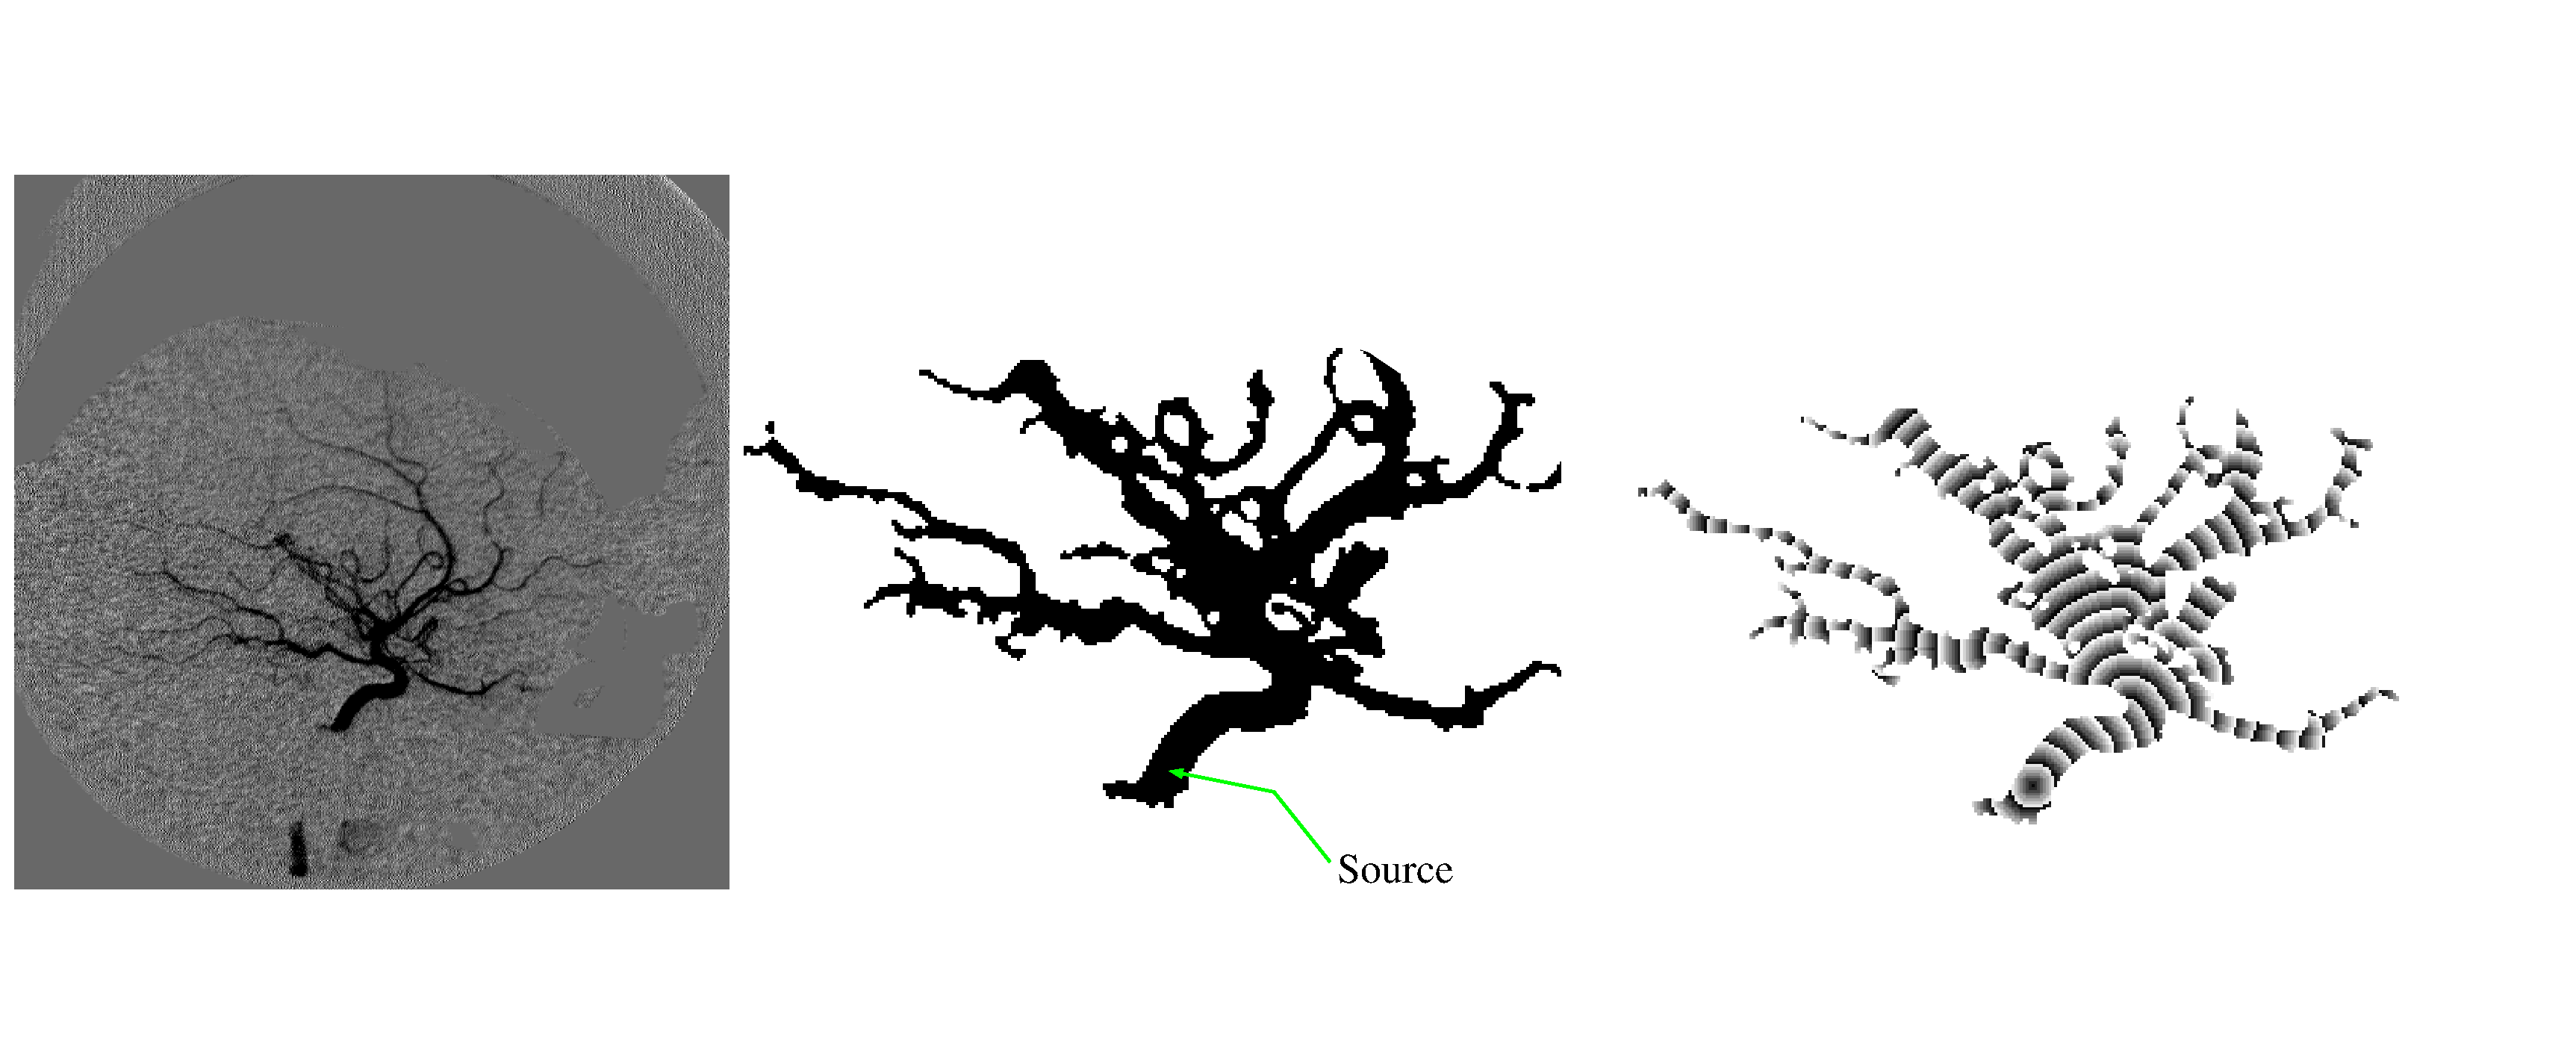
\includegraphics[width=7.5cm]{angio}
    \caption{Application of the geodesic labelling in medical imaging: {\it left} An angiography image,
      {\it middle} binary image when blood vessels are segmented and {\it right} the geodesic
      labelling.}
    \label{angio}
  \end{center}
\end{figure}


Using  this  geodesic distance algorithm,  we naturally  would like to
apply  this algorithm to compute  the discrete Voronoi  diagram or the
Euclidean distance transform just considering multiple sources.  Since
this  algorithm use a  local  propagation scheme (as the  Cuisenaire's
algorithm \cite{cuisenaire}),  the   classical Danielsson's algorithm
errors are not solved in this approach. Hence, this algorithm presents
a solution to this problem but errors may occur.



\section{On an extension to 3D domains}
\label{section3D}
%etape suivant c'est la version3D pour visi et geodes en 3D et surtout
%pour def et algo de geodes sur des surfaces
%
% 1 extension avec Bresenham3D et debled 3D des geodes de Soille 
% ca  donne visi et geodes
%
% discussion pour des visi dcoeurjo : probleme avec giq meme avec
% vis restreinte
%

A natural extension of these algorithms is to define both visibility
and geodesic paths in higher dimensions and in particular to three
dimensional domains. Hence, in the following we consider the domain
$\mathcal{D}$ as a 26-connected set of voxels and $\bar{\mathcal{D}}$
the set of obstacle voxels.

In the case of mask based metrics, efficient algorithms exist for the
geodesic distance labelling since the problem can be shifted to a classical
shortest path on a weighted graph as in 2D \cite{kiryati93,sven}. 


In our proposal of visibility based geodesic paths, definitions of the
visibility are the same as in dimension 2, {\it i.e.}, two points in $\mathcal{D}$
 are said  to be visible if  and only if there
exists at least one 26-connected 3D  discrete straight segment joining
these points  whose voxels  belong to the  domain.  In the literature,
many algorithms   exist     for drawing  3D lines   between   points
\cite{bres65,KAU86,AMA87}.  Based on an  arithmetical definition of 3D
discrete straight lines  \cite{FIG95}, recognition and segmentation of
a     3D curve into  digital    straight   segments algorithms   exist
\cite{3Dnss}.

For   the visibility labelling   in   non-convex domains, the  problem
becomes more complex than  in 2D. As  a matter of fact,  the parameter
space analysis of  a 3D  straight line  is  more  complicated and  the
visibility test  considering complementary  of  domains associated  to
voxels  is not so  direct.  To illustrate  these problems, we consider
the weak visibility in 3D.  Hence, the visibility domain associated to
two points $s$ and  $t$, is the  set of Euclidean straight lines going
through $s$ whose  digitization  contains    $t$.  Without loss     of
generality, we consider  $\vec{st}=(a,b,c)^T$  such that $a\geq  b\geq
c>0$.   So, in the primal  space,  the Euclidean  3D straight lines go
through $s$ and cross the square centered on $t$ of size 1 parallel to
the  $yz$-plane (cf figure \ref{cone3D}-a).   Let us  consider now the
obstacle voxels and their perspective projections of center $s$ on the
$yz$-plane containing $t$. Hence, the visibility  domain is the set of
lines going through $s$  and crossing the projected square  associated
to $t$ at a point not covered by  obstacle projected square (cf figure
\ref{cone3D}-b).  During this weak visibility test, the number of {\it
blocking  voxels}   cannot  be   bounded  by a    constant  as in  2D.
Furthermore, an efficient algorithm to detect if there exists a subset
of the projected square of $t$ which is not covered by blocking voxels
is not straightforward.

\begin{figure}[htb]
  \begin{center}
    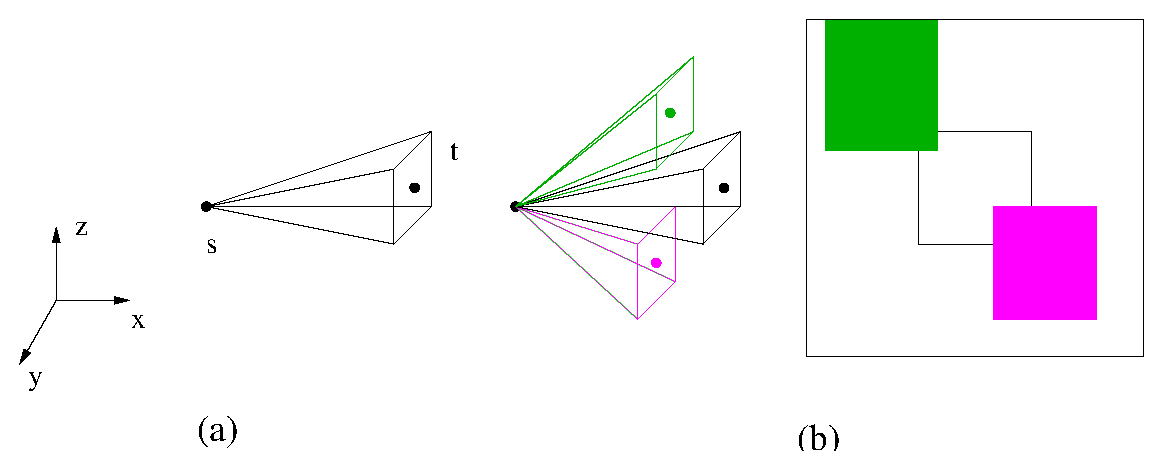
\includegraphics[width=7.5cm]{cone3D}
   \caption{Illustration of the weak visibility ib 3D: (a) primal space
    illustration of the visibility domain, (b) visibility test, gray
    pyramids represent obstacle visibility domains and their
    projection on the $yz$-plane containing $t$.}
   \label{cone3D}
\end{center}
\end{figure}

Despite these difficulties, we can present a first solution based on a
3D          generalization        of   the        Soille's    approach
\cite{soille91,soille94,soillebook}.  In that  case, the   visibility
test between $s$ and $t$ is the  following: we construct a 3D discrete
straight segment  between $s$  and $t$  using  a 3D  generalisation of
Bresenham's algorithm  \cite{AMA87,3Dnss}  and we   verify that   all
pixels of this segment  belong to $\mathcal{D}$. Using this visibility
labelling, we can use the same data structure as  in the 2D case based
on Bucket list  and thus we can  design a geodesic  distance labelling
algorithm.  Note that  the  computational  cost of this   algorithm is
high: the  visibility  test is  done in $O(d)$   where $d$ denotes the
diameter of $\mathcal{D}$ and then we have a global cost in $O(nd)$ if
$n$ is the number of voxels in $\mathcal{D}$.

Figure \ref{vis3d} presents an illustration of the visibility
labelling algorithm considering non-convex 3D domains. Figure
\ref{geodes3d} illustrates the geodesic distance labelling using a
circular gray scale map. If we consider a discrete domain $\mathcal{D}$ as a voxel based discrete surface, 
we can compute geodesic distances on these objects (see figure
\ref{surface_geodes3d}).

\begin{figure}[htb]
  \begin{center}
    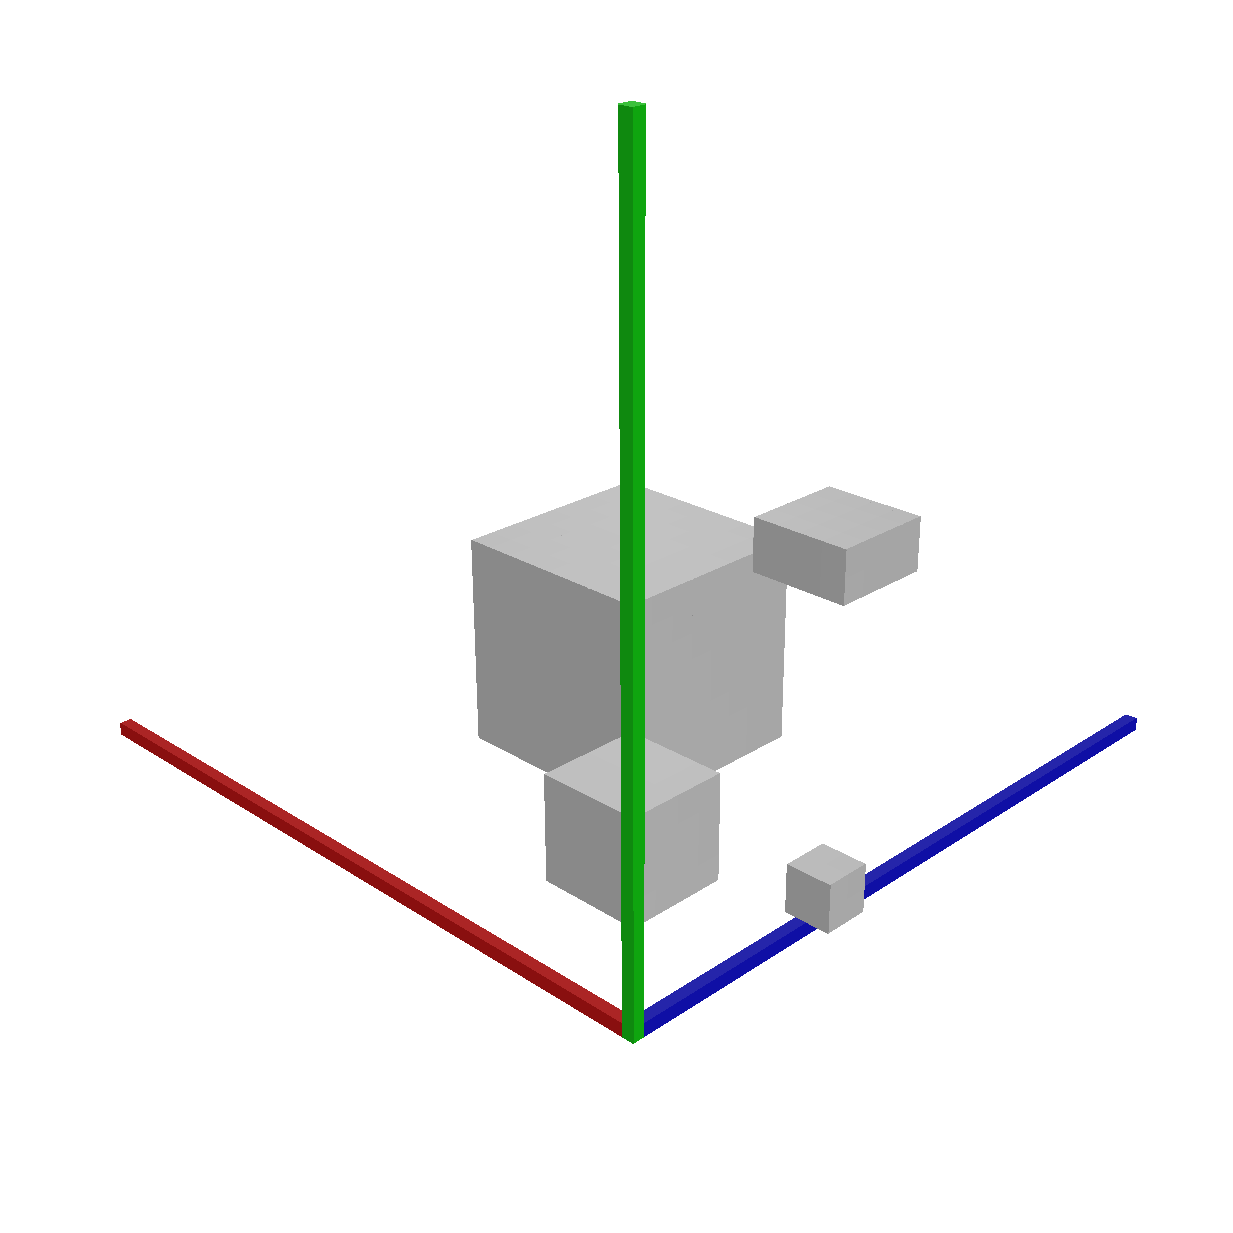
\includegraphics[width=3.5cm]{cone_obs}
    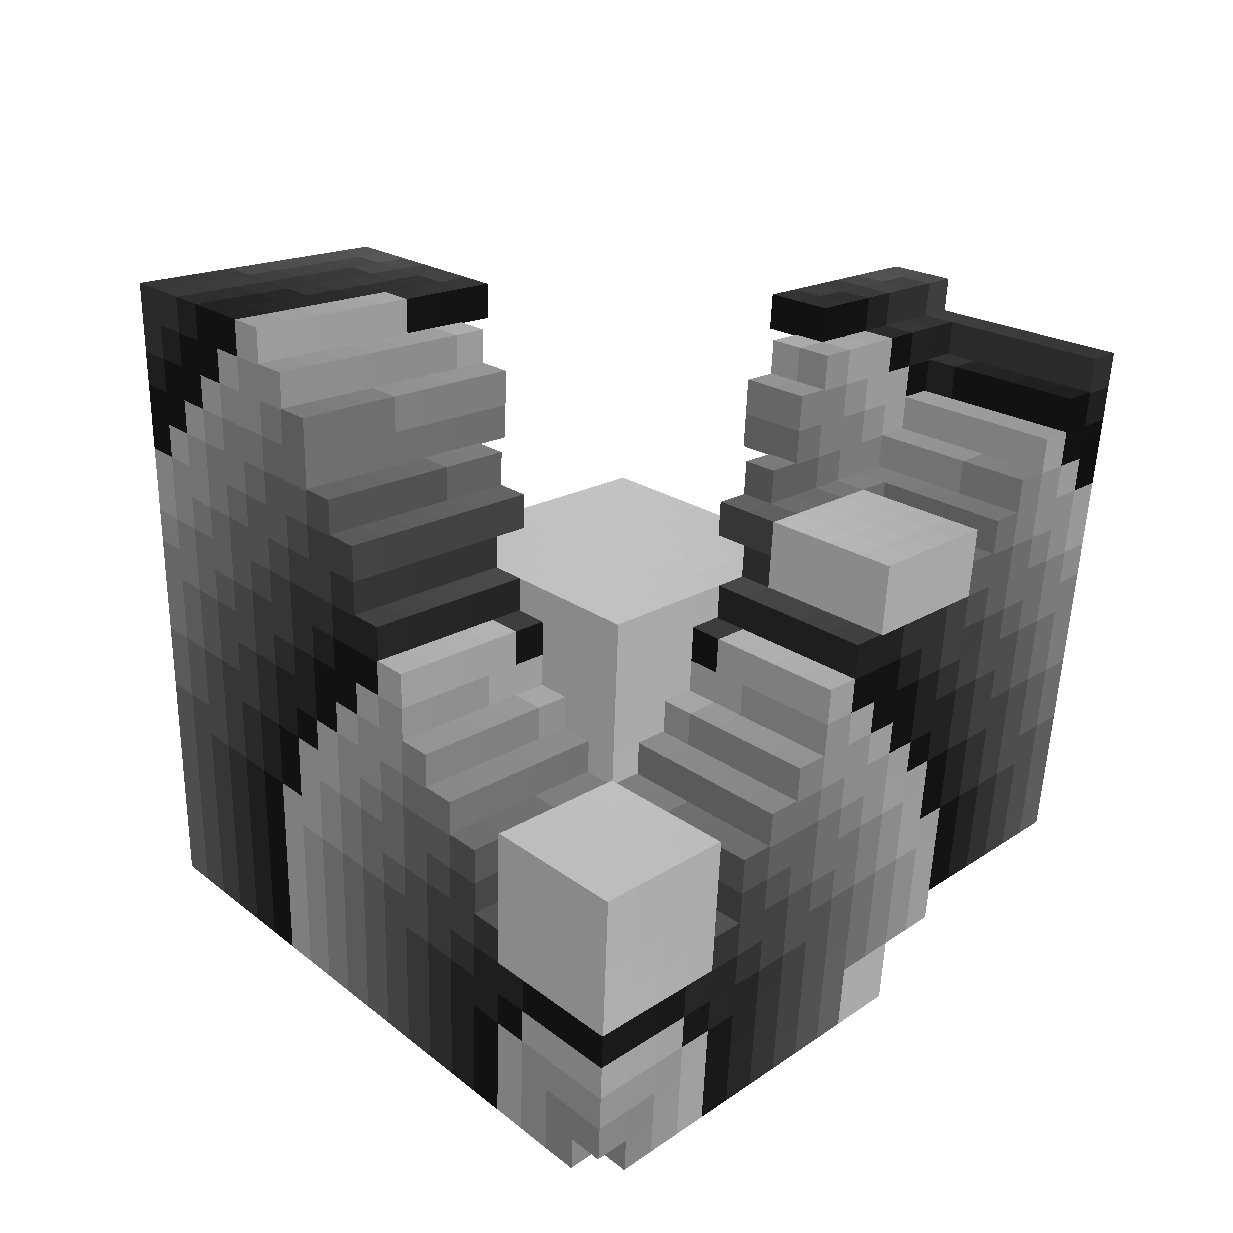
\includegraphics[width=3.5cm]{cone}
    \caption{Visibility labelling: {\it left} obstacles of a 3D
      domain, {\it right} result of the visibility labelling  where
      the source point is the lower corner.}
  \label{vis3d}
\end{center}
\end{figure}

\begin{figure}[htb]
  \begin{center}
    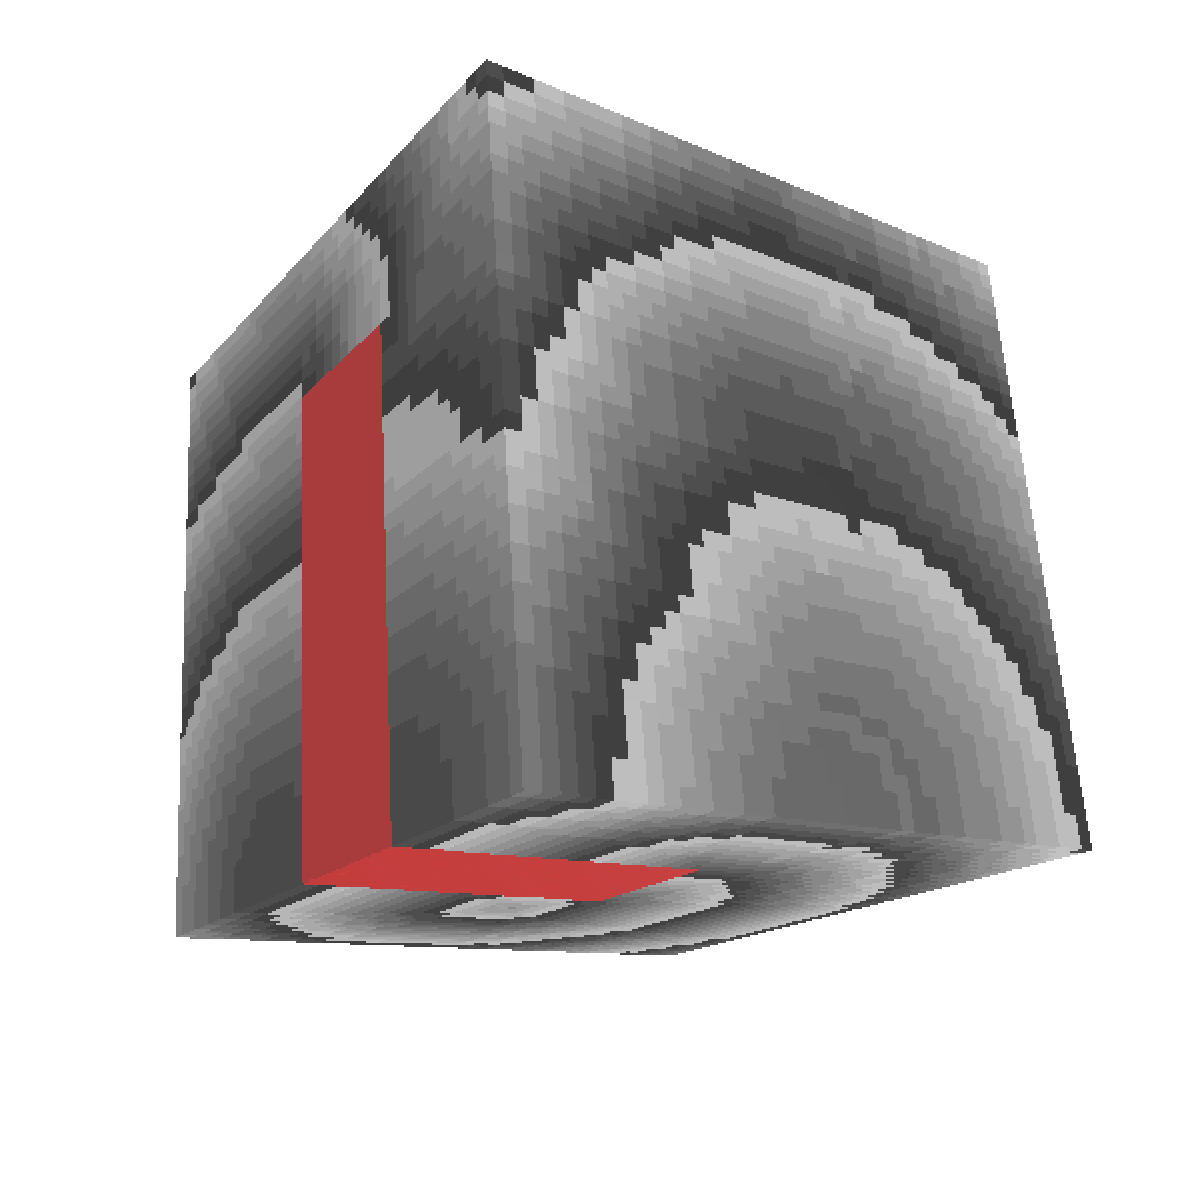
\includegraphics[width=3.5cm]{obstacle}
    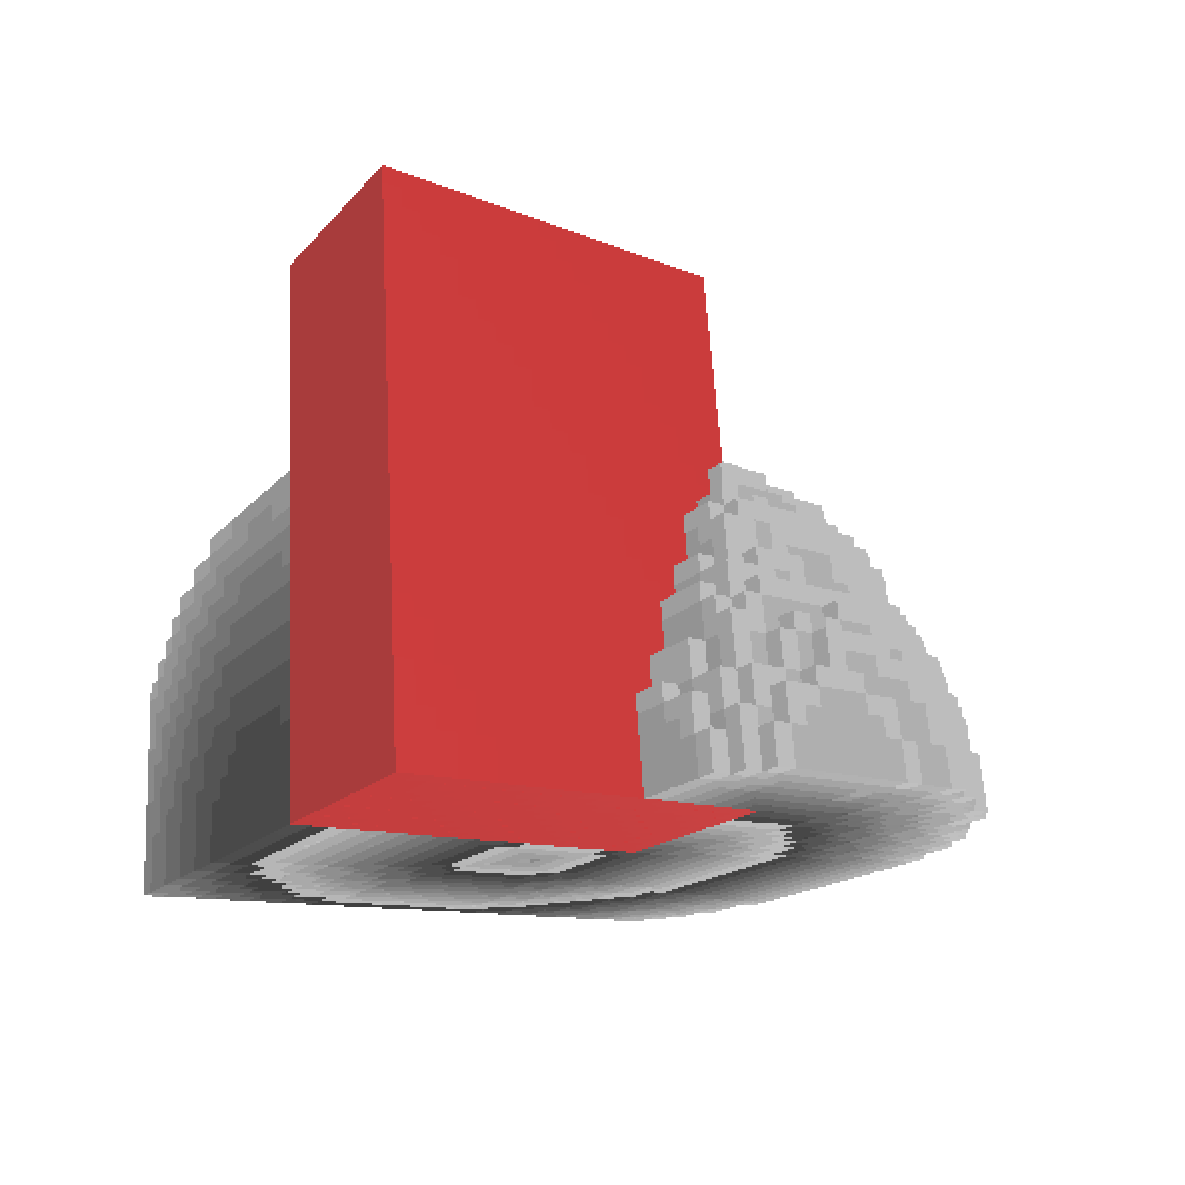
\includegraphics[width=3.5cm]{obstacle_onde}
    \caption{Geodesic labelling on a 3D domain with obstacle: {\it left}
    global labelling, {\it right} result when the distances are thresholded.}
  \label{geodes3d}
\end{center}
\end{figure}

\begin{figure}[htb]
  \begin{center}
%   \subfigure[]{ 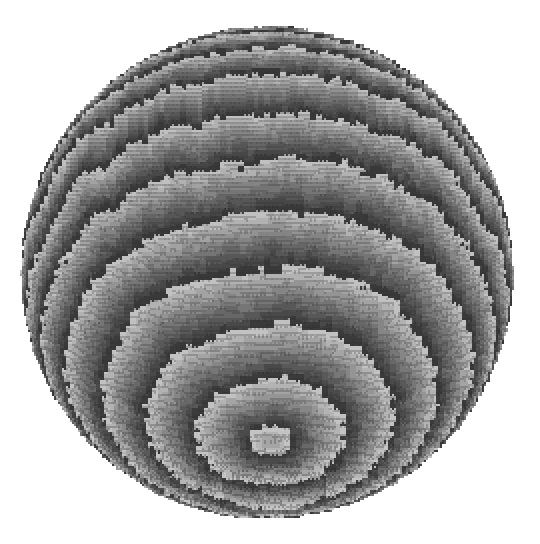
\includegraphics[width=3cm]{sphere_red}}
%   \subfigure[]{ 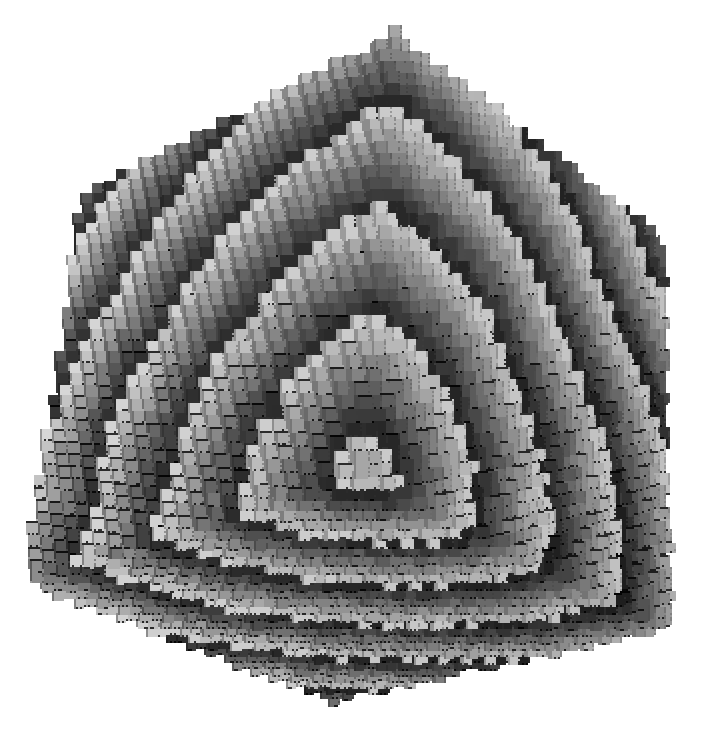
\includegraphics[width=3cm]{cube}}
%   \subfigure[]{ 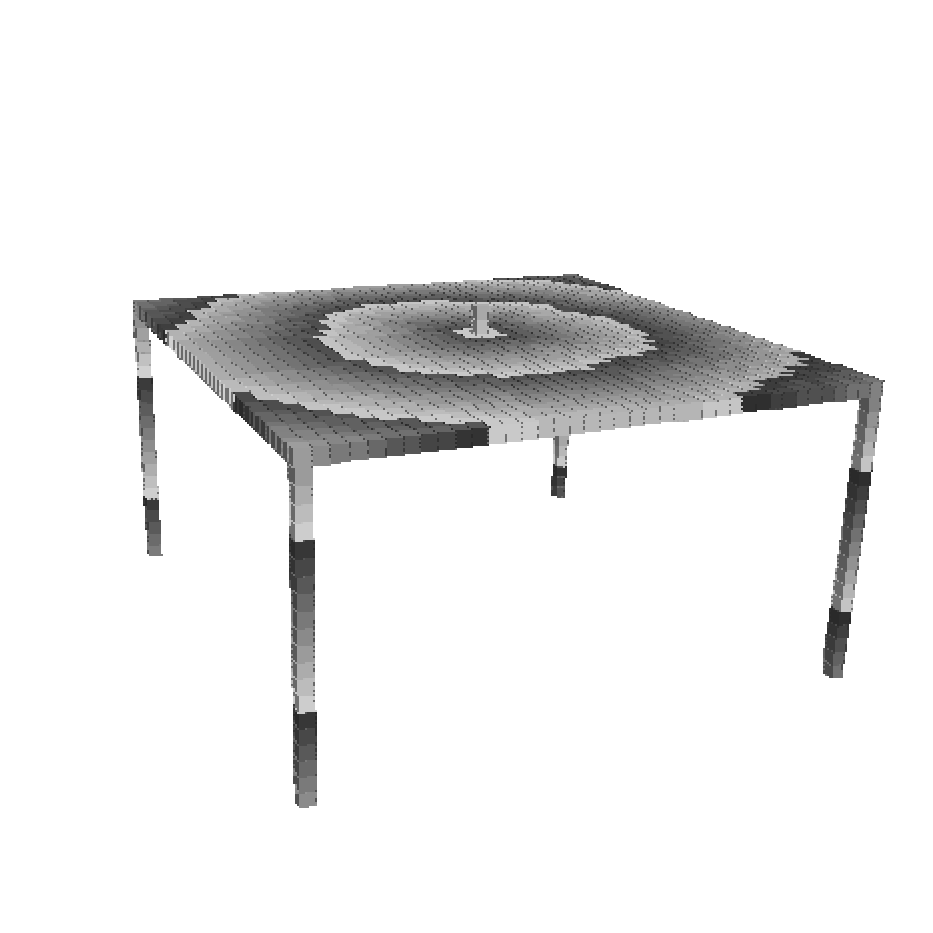
\includegraphics[height=3cm]{table}}
    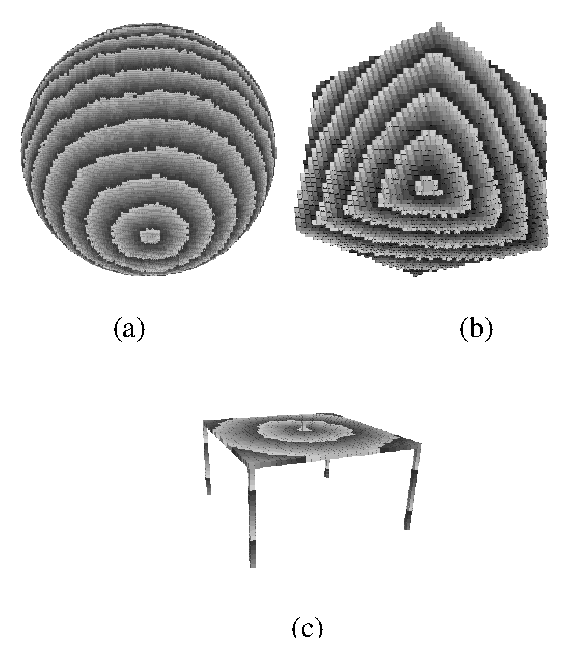
\includegraphics[width=6cm]{surfaces}
   \caption{(a) Geodesic distance labelling on a discrete sphere
      surface, (b) on a  rotated  cube surface and (c) on a table-like
      surface (the source point is in the middle of the plate) }
  \label{surface_geodes3d}
\end{center}
\end{figure}
\section{Conclusion}

In  this  article, we   have presented a   discrete  definition of the
visibility  well-known in   classical  computational  geometry.   This
definition   is  based on well  known   discrete objects  (DSS) and is
computed   only  with integers.  Based on   this  definition,  we have
presented algorithms to  solve several problems: if  we want to decide
if there exists at least one DSS between two pixels,  we have a linear
cost in the number of obstacle pixels $O(m)$~; if we want to label all
pixels in a domain which are  visible from a  source point, we have an
algorithm in $O(nm)$.  Using the weak visibility definition, we reduce
the complexity of  both  algorithms  respectively to  $O(log(m))$  and
$O(nlog(m))$.    We also have   presented  a  definition   of discrete
geodesic paths and an algorithm  that computes the geodesic distance of
each point in the domain according to a source.

This article also introduces open problems:  is it possible to find an
efficient data structure for  the straightforward visibility algorithm
? How  to  generalize this approach  for 3D  domains and for  discrete
surfaces  ?   For this  last  problem, we have presented a first solution but
 more efficient algorithms similar to the 2D ones  are expected.




\bibliography{geodesiques} 
\end{document}
% LocalWords:  literature
